\section{Functional Specification}

This section provides a comprehensive overview of the system's functionality. It includes a use case diagram illustrating the system's interactions and a detailed textual description of each use case.

\subsection{Use Case Diagram}

Figure \ref{fig:Sprint 2 Use Case Diagram} offers us an overview by presenting a visual description of the functional
behaviour of our tool during the second sprint. This diagram sums up the interactions among the actors and the
diverse use cases within the system.

\begin{figure}[ht]
	\centering
	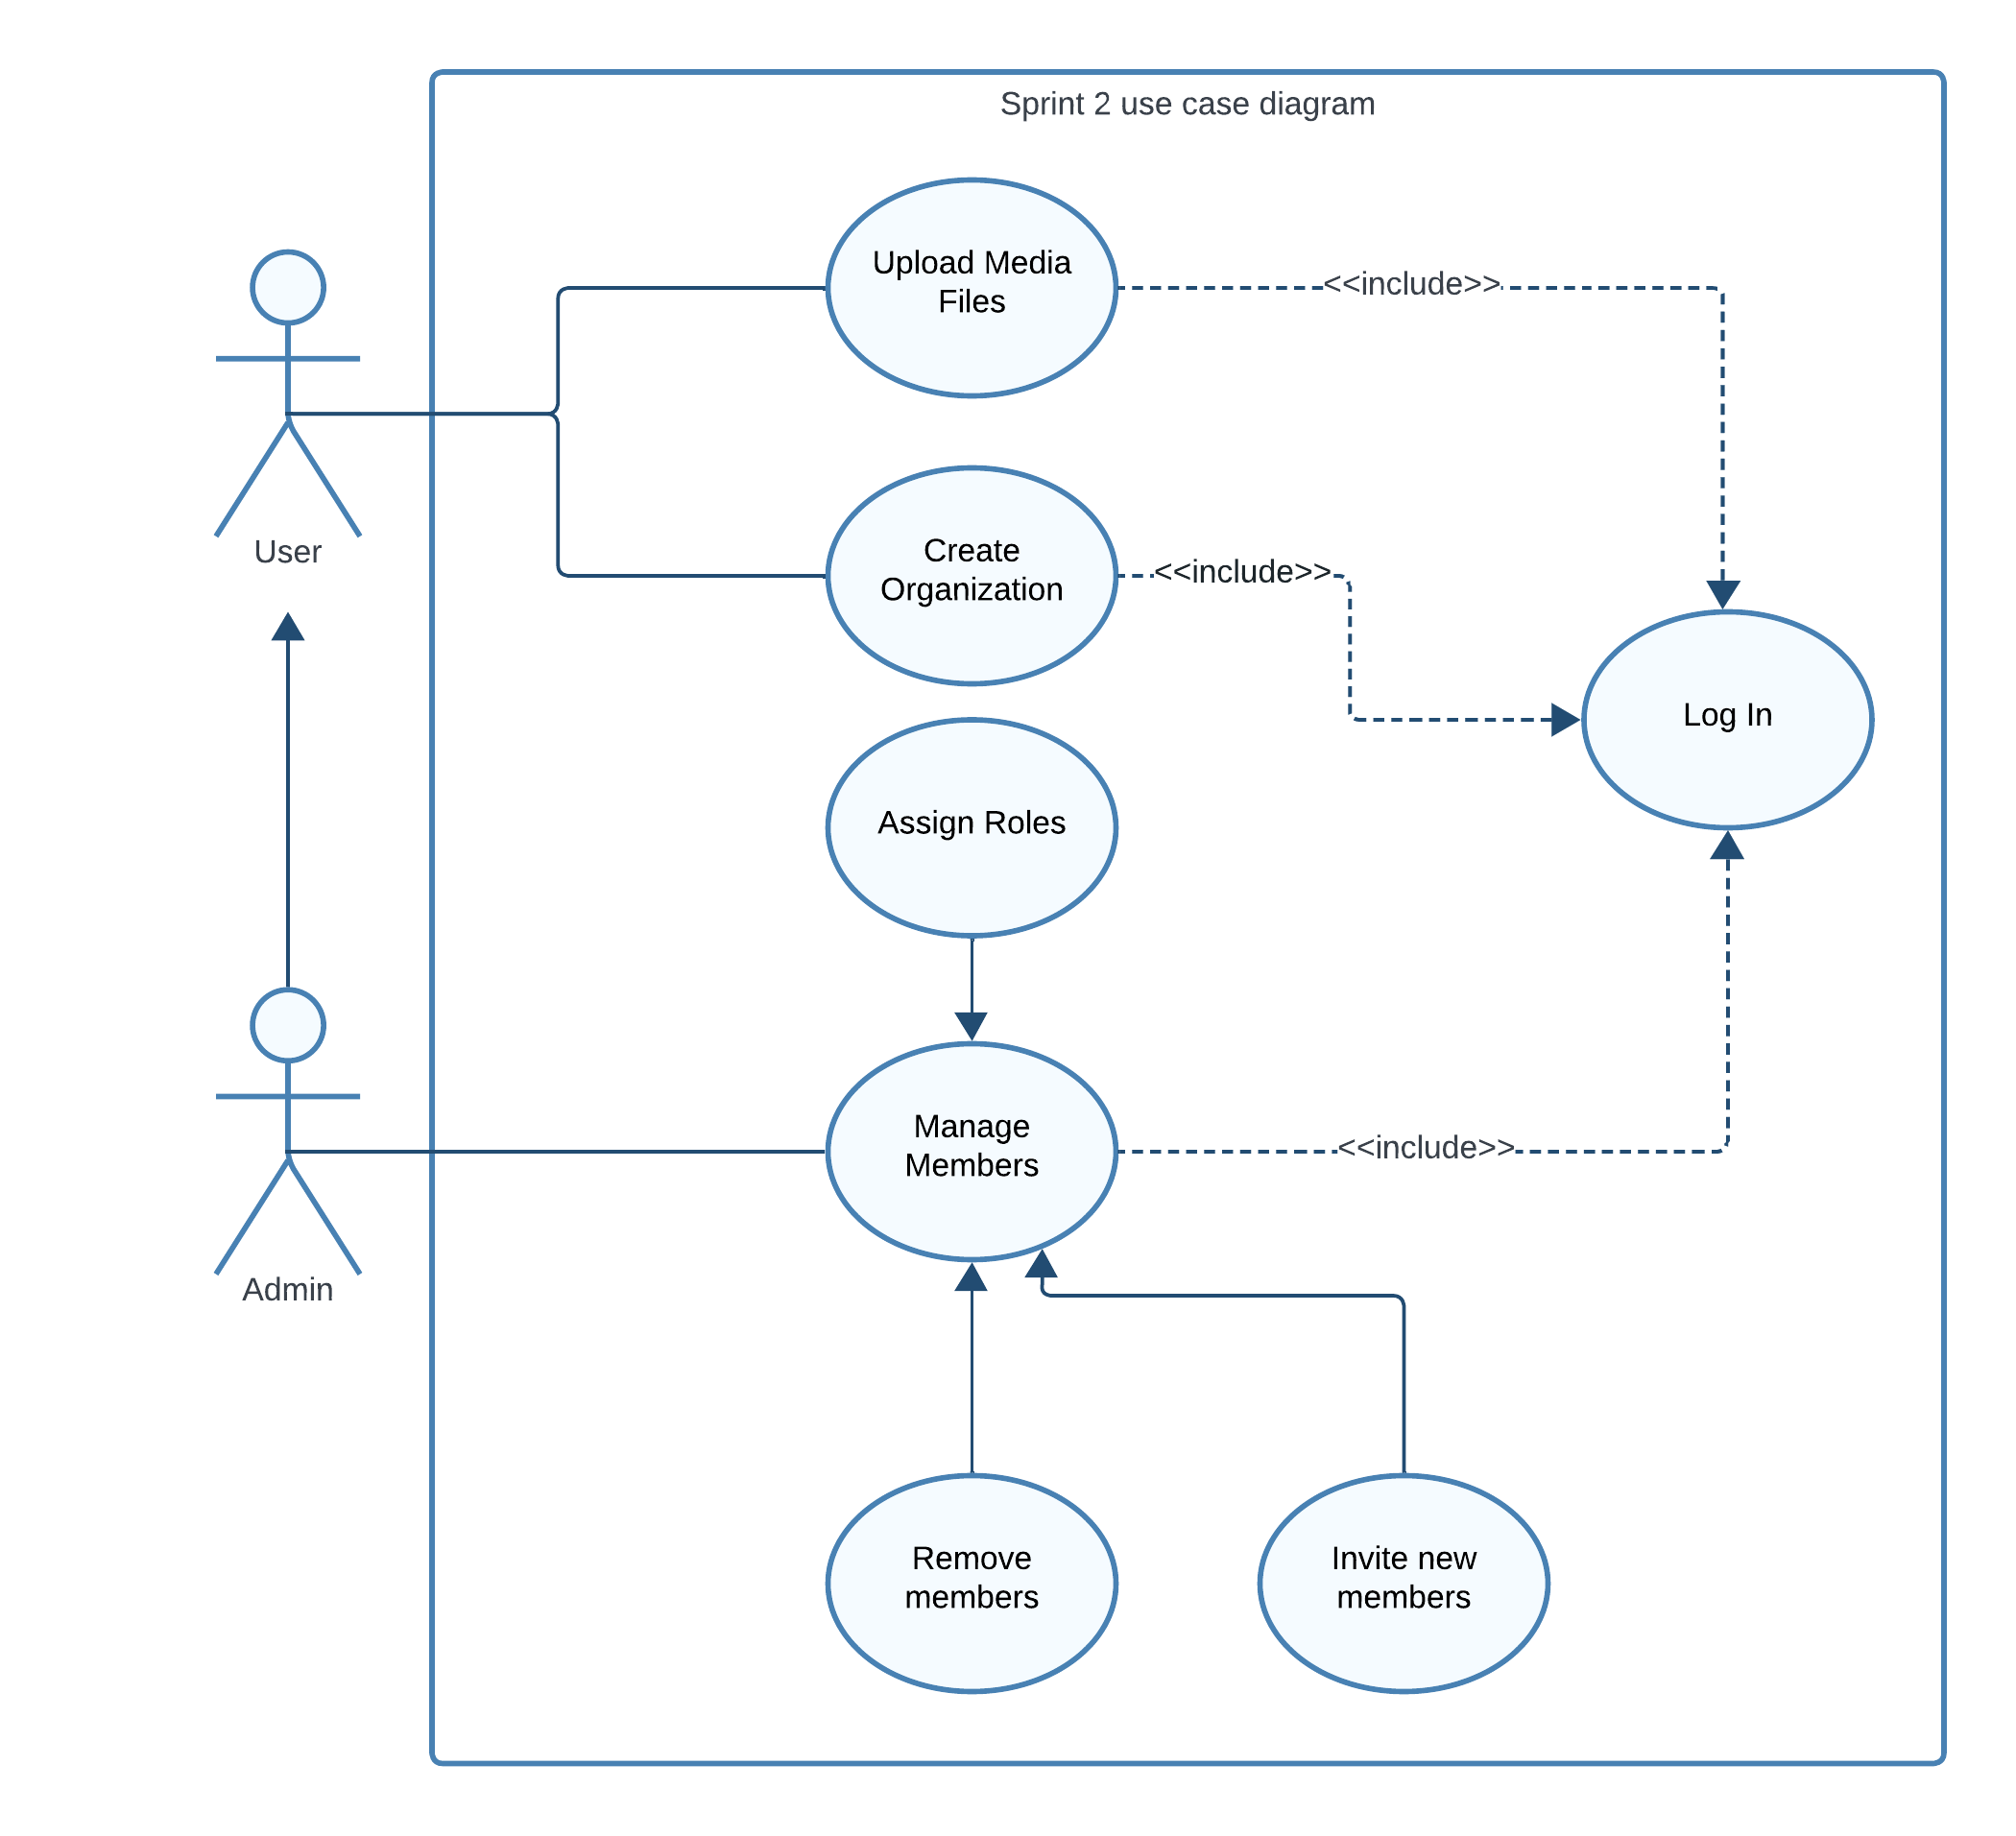
\includegraphics[width=\linewidth]{Images/sprint2/use case diagram.png}
	\caption{Sprint 2 Use Case Diagram}
	\label{fig:Sprint 2 Use Case Diagram}
\end{figure}

\clearpage

\subsection{Textual Description of Use Cases}
The following tables provide a detailed description of the use cases. This includes the actor, the goal of the use case, the preconditions, the basic flow, the alternative flows, and the postconditions.

\subsubsection{Use Case 1: Upload Media Files}

Table \ref{tab:Use Case 1 Upload Media Files} presents a textual description of the use case: Upload Media Files.

\begin{table}[ht]
	\centering
	\begin{tabularx}{\textwidth}{|l|X|}
		\hline
		\textbf{Actor}             & User, admin                                                                      \\
		\hline
		\textbf{Goal}              & To upload media files (e.g., images, videos) to the system                       \\
		\hline
		\textbf{Preconditions}     & The user is logged in and has access to the media upload feature                 \\
		\hline
		\textbf{Basic Flow}        & 1. The user selects the media files they want to upload                          \\
		                           & 2. The system validates the file format and size                                 \\
		                           & 3. The system stores the uploaded files in the appropriate location              \\
		\hline
		\textbf{Alternative Flows} & If the file format or size is invalid, the system displays an error message      \\
		\hline
		\textbf{Postconditions}    & The media files are successfully uploaded and associated with the user's account \\
		\hline
	\end{tabularx}
	\caption{Use Case 1: Upload Media Files}
	\label{tab:Use Case 1 Upload Media Files}
\end{table}

\subsubsection{Use Case 2: Create Organizations}

Table \ref{tab:Use Case 2 Create Organizations} presents a textual description of the use case: Create Organizations.

\begin{table}[ht]
	\centering
	\begin{tabularx}{\textwidth}{|l|X|}
		\hline
		\textbf{Actor}             & User, Admin                                                                                       \\
		\hline
		\textbf{Goal}              & To create new organizations within the system                                                     \\
		\hline
		\textbf{Preconditions}     & The user or admin is logged in and has the necessary permissions to create organizations          \\
		\hline
		\textbf{Basic Flow}        & 1. The user or admin selects the option to create a new organization                              \\
		                           & 2. The system prompts for organization details                                                    \\
		                           & 3. The user or admin provides the required information                                            \\
		                           & 4. The system validates the input and creates the organization                                    \\
		\hline
		\textbf{Alternative Flows} & If the provided organization details are incomplete or invalid, the system shows an error message \\
		\hline
		\textbf{Postconditions}    & A new organization is successfully created and added to the system                                \\
		\hline
	\end{tabularx}
	\caption{Use Case 2: Create Organizations}
	\label{tab:Use Case 2 Create Organizations}
\end{table}

\subsubsection{Use Case 3: Assign Roles to Users}

Table \ref{tab:Use Case 3 Assign Roles to Users} presents a textual description of the use case: Assign Roles to Users.

\begin{table}[ht]
	\centering
	\begin{tabularx}{\textwidth}{|l|X|}
		\hline
		\textbf{Actor}             & Admin                                                                                                                        \\
		\hline
		\textbf{Goal}              & To assign specific roles to users within an organization                                                                     \\
		\hline
		\textbf{Preconditions}     & The admin is logged in and has the necessary permissions to manage roles, targeted user already a member of the organization \\
		\hline
		\textbf{Basic Flow}        & 1. The admin choses a user within an organization                                                                            \\
		                           & 2. The system displays available roles (e.g., member, admin)                                                                 \\
		                           & 3. The admin assigns a role to the chosen user                                                                               \\
		\hline
		\textbf{Alternative Flows} & If the admin selects an invalid user or the roles are not available, the system shows an error message                       \\
		\hline
		\textbf{Postconditions}    & The user is assigned the specified roles within the organization                                                             \\
		\hline
	\end{tabularx}
	\caption{Use Case 3: Assign Roles to Users}
	\label{tab:Use Case 3 Assign Roles to Users}
\end{table}

\subsubsection{Use Case 4: Send Invitation to Join Organization}

Table \ref{tab:Use Case 4 Send Invitation} presents a textual description of the use case: Send Invitation to Join Organization via Email.

\begin{table}[ht]
	\centering
	\begin{tabularx}{\textwidth}{|l|X|}
		\hline
		\textbf{Actor}             & Admin                                                                                                                                  \\
		\hline
		\textbf{Goal}              & To invite users to join an organization by sending email invitations                                                                   \\
		\hline
		\textbf{Preconditions}     & The admin is logged in and has the necessary permissions to manage organization invitations, the targeted user already have an account \\
		\hline
		\textbf{Basic Flow}        & 1. The admin enters users emails.                                                                                                      \\
		                           & 2. The system generates invitation emails with unique links.                                                                           \\
		                           & 3. The admin sends the invitation emails to the selected users.                                                                        \\
		\hline
		\textbf{Alternative Flows} & If there are no eligible users to invite or if the email sending fails, the system shows an error message.                             \\
		\hline
		\textbf{Postconditions}    & Invitation emails are successfully sent to the selected users.                                                                         \\
		\hline
	\end{tabularx}
	\caption{Use Case 4: Send Invitation to Join Organization via Email}
	\label{tab:Use Case 4 Send Invitation}
\end{table}

\subsubsection{Use Case 5: Remove User from an Organization}

Table \ref{tab:Use Case 5 Remove User from an Organization} presents a textual description of the use case: Remove User from an Organization.
\begin{table}[ht]
	\centering
	\begin{tabularx}{\textwidth}{|l|X|}
		\hline
		\textbf{Actor}             & Admin                                                                                                                                        \\
		\hline
		\textbf{Goal}              & To remove a user from an organization                                                                                                        \\
		\hline
		\textbf{Preconditions}     & The admin is logged in and has the necessary permissions to manage users within the organization. The targeted user is a member of the organization. \\
		\hline
		\textbf{Basic Flow}        & 1. The admin selects a user within the organization and clicks on the remove icon.                                                           \\
		                           & 2. The system changes the status of the selected user to inactive and removes their association with the organization.                       \\
		\hline
		\textbf{Alternative Flows} & If the removal process fails due to a system error, the system notifies the admin and logs the error.                                      \\
		\hline    
		\textbf{Postconditions}    & The user is successfully removed from the organization, and their status is updated to inactive.                                             \\
		\hline
	\end{tabularx}
	\caption{Use Case 5: Remove User from an Organization}
	\label{tab:Use Case 5 Remove User from an Organization}
\end{table}
